\documentclass[10pt,a4paper]{article}
% Note de 8 pages (17/11/2026). Chiffres : note8p/sorties/*.json et *.md ; bouclage : calculs/bouclage.py ;
% figures : charte.py. Annexe technique séparée : annexe_technique.tex.
% Préambule de la note de 8 pages et de son annexe technique (note8p/).
\usepackage[T1]{fontenc}
\usepackage[utf8]{inputenc}
\usepackage{lmodern}
\usepackage[french]{babel}
\usepackage[a4paper,left=2.1cm,right=2.1cm,top=1.9cm,bottom=2.0cm]{geometry}
\usepackage{graphicx}
\usepackage{booktabs,tabularx,array}
\usepackage{xcolor}
\usepackage{titlesec}
\usepackage[labelfont=bf,labelsep=period,font=small,singlelinecheck=false,justification=raggedright,skip=3pt]{caption}
\usepackage{fancyhdr}
\usepackage{enumitem}
\usepackage{microtype}
\usepackage{textcomp}
\usepackage{amsmath}
\usepackage{wrapfig}
\providecommand{\euro}{\texteuro}
\usepackage[hidelinks]{hyperref}

\definecolor{encre}{HTML}{1A1A1A}
\definecolor{bleu}{HTML}{173F8A}
\definecolor{brique}{HTML}{B8642A}
\definecolor{gris}{HTML}{555555}

\titleformat{\section}{\normalfont\large\bfseries\color{bleu}}{}{0em}{}
\titleformat{\subsection}{\normalfont\normalsize\bfseries\color{bleu}}{}{0em}{}
\titlespacing*{\section}{0pt}{1.6ex plus .6ex minus .2ex}{0.6ex plus .2ex}
\titlespacing*{\subsection}{0pt}{1.2ex plus .5ex minus .2ex}{0.4ex plus .1ex}

\pagestyle{fancy}
\fancyhf{}
\renewcommand{\headrulewidth}{0pt}
\fancyfoot[R]{\small\color{gris}\thepage}
\fancyfoot[L]{\small\color{gris}Taxer mieux plutôt que davantage}

\setlength{\parindent}{0pt}
\setlength{\parskip}{0.45em}
\linespread{1.02}
\setlist{itemsep=1pt,topsep=1pt,parsep=0pt,leftmargin=1.2em}
\setlength{\textfloatsep}{8pt plus 2pt minus 2pt}
\setlength{\floatsep}{6pt plus 2pt minus 2pt}
\renewcommand{\topfraction}{0.85}\renewcommand{\bottomfraction}{0.7}
\renewcommand{\textfraction}{0.12}\renewcommand{\floatpagefraction}{0.8}

% \graphique{fichier}{titre-message}{label} : figure pleine largeur, source composée en petit sous l'image.
\newcommand{\graphique}[3]{%
  \begin{figure}[!htbp]\centering
  \caption{#2}\label{#3}\vspace{1pt}
  \includegraphics[width=\linewidth]{figures/#1.pdf}\par\vspace{1pt}
  {\raggedright\scriptsize\color{gris}\input{figures/#1_source.tex}\par}
  \end{figure}}
% \deuxgraphiques{f1}{titre1}{lab1}{f2}{titre2}{lab2} : deux figures demi-largeur côte à côte.
\newcommand{\deuxgraphiques}[6]{%
  \begin{figure}[!htbp]
  \begin{minipage}[t]{0.485\linewidth}\caption{#2}\label{#3}\vspace{1pt}
  \includegraphics[width=\linewidth]{figures/#1.pdf}\par
  {\raggedright\scriptsize\color{gris}\input{figures/#1_source.tex}\par}\end{minipage}\hfill
  \begin{minipage}[t]{0.485\linewidth}\caption{#5}\label{#6}\vspace{1pt}
  \includegraphics[width=\linewidth]{figures/#4.pdf}\par
  {\raggedright\scriptsize\color{gris}\input{figures/#4_source.tex}\par}\end{minipage}
  \end{figure}}

\newenvironment{encadre}[1]
  {\par\smallskip\noindent\begin{minipage}{\linewidth}\color{encre}\setlength{\parskip}{0.3em}%
   \hrule height 0.6pt\vspace{4pt}{\footnotesize\bfseries\color{bleu}\MakeUppercase{#1}}\par\small}
  {\par\vspace{3pt}\hrule height 0.3pt\end{minipage}\par\smallskip}

\DeclareUnicodeCharacter{2212}{\ensuremath{-}}
\DeclareUnicodeCharacter{2248}{\ensuremath{\approx}}
\DeclareUnicodeCharacter{00D7}{\ensuremath{\times}}
\DeclareUnicodeCharacter{2192}{\ensuremath{\rightarrow}}
\DeclareUnicodeCharacter{2264}{\ensuremath{\leq}}
\DeclareUnicodeCharacter{2265}{\ensuremath{\geq}}
\DeclareUnicodeCharacter{202F}{\,}
\DeclareUnicodeCharacter{2009}{\,}
\DeclareUnicodeCharacter{03C3}{\ensuremath{\sigma}}
\DeclareUnicodeCharacter{03C4}{\ensuremath{\tau}}
\DeclareUnicodeCharacter{03C1}{\ensuremath{\rho}}
\DeclareUnicodeCharacter{03B5}{\ensuremath{\varepsilon}}
\DeclareUnicodeCharacter{03B4}{\ensuremath{\delta}}
\DeclareUnicodeCharacter{03BB}{\ensuremath{\lambda}}
\DeclareUnicodeCharacter{00B2}{\textsuperscript{2}}

% \graphiquemarge{fichier}{titre}{label} : figure demi-largeur habillée par le texte (à placer en début de paragraphe).
\newcommand{\graphiquemarge}[3]{%
  \begin{wrapfigure}{r}{0.47\linewidth}\vspace{-10pt}
  \captionsetup{type=figure}\caption{#2}\label{#3}\vspace{1pt}
  \includegraphics[width=\linewidth]{figures/#1.pdf}\par
  {\raggedright\scriptsize\color{gris}\input{figures/#1_source.tex}\par}\vspace{-6pt}
  \end{wrapfigure}}


\begin{document}

{\footnotesize\color{brique}\bfseries NOTE DE POLITIQUE ÉCONOMIQUE\quad·\quad NOVEMBRE 2026\par}
\vspace{4pt}
{\fontsize{20}{24}\selectfont\bfseries\color{bleu}Taxer mieux plutôt que davantage\par}
\vspace{3pt}
{\large Quatre réformes pour une fiscalité qui récompense le travail, l'investissement et la mobilité, sans un euro de
dette en plus\par}
\vspace{5pt}
{\color{bleu}\hrule height 1pt}
\vspace{2pt}

\section{Taxer moins ce qui crée la richesse}

Le débat fiscal français porte presque toujours sur deux questions : combien faut-il prélever, et sur qui ? Il en existe
une troisième, au moins aussi importante pour notre prospérité : prélevons-nous de la bonne manière ?

Tous les impôts n'ont pas le même coût. Taxer l'augmentation d'un salarié, la machine d'une PME ou la construction d'un
immeuble décourage précisément ce qui crée de la richesse. Taxer la valeur d'un terrain ne décourage rien : le terrain
ne peut ni fuir, ni travailler moins, ni se cacher. Or notre système fiscal pénalise souvent ce que nous voudrions
encourager. Nous voulons plus de travail, mais un salarié qui passe de 1,1 à 1,8 Smic voit près d'un quart de chaque
euro supplémentaire prélevé, sans même compter les cotisations. Nous voulons des familles qui déménagent pour un meilleur
emploi, mais l'État prélève près de 6~\% du prix à chaque achat. Nous voulons des entreprises qui grandissent, mais
nous leur accordons un taux d'impôt réduit tant qu'elles restent petites. Nous voulons que le capital circule, mais
l'impôt sur une plus-value disparaît si son détenteur la garde jusqu'à sa mort.

Et si nous commencions par corriger ces contradictions ? Cette note propose quatre réformes, à niveau de prélèvements
constant et sans dette de transition :
\begin{itemize}
\item \textbf{un nouvel impôt sur le revenu}, qui fusionne l'IR, la CSG et la CRDS : individuel, le même pour un
salaire et pour une pension, à quatre taux de 5 à 45~\% (tableau~\ref{tab:bareme}), avec une franchise de 6\,000~€ par enfant ;
\item \textbf{une fiscalité immobilière tournée vers le sol} : droits de mutation divisés par deux, taxe foncière
assise surtout sur la valeur des terrains, et 15~Md€ de recettes foncières nouvelles ;
\item \textbf{un impôt sur les sociétés qui favorise l'investissement} : fin du taux réduit des petites entreprises,
déduction immédiate de la moitié des achats d'équipements, taux normal ramené de 25 à 22,5~\% ;
\item \textbf{une fiscalité du capital stable}, qui garde le prélèvement forfaitaire unique mais cesse d'effacer les
plus-values à la transmission.
\end{itemize}
Notre ambition n'est pas la fiscalité parfaite des manuels. Nous retenons des instruments simples, déjà pratiqués
ailleurs, et nous écartons ceux qui coûteraient plusieurs milliards pour un effet incertain. Les gagnants sont les
actifs, les familles, ceux qui déménagent et les entreprises qui investissent. Les perdants existent, et nous les
montrons : les retraités modestes et moyens, les couples à un seul revenu élevé, les propriétaires de terrains chers,
les petites sociétés qui n'investissent pas.

\section{Travailler davantage doit rapporter davantage}

Prenons un salarié payé 2\,000~€ net par mois qui obtient une augmentation de 200~€. Sur les 2\,689~€ de revenu
supplémentaire qu'elle lui apporte chaque année après cotisations, l'IR et la CSG lui en prennent 647, soit 24~\%.
Pourquoi autant, à ce niveau de salaire ? Parce qu'il entre précisément dans l'impôt sur le revenu, et que la
« décote », censée adoucir cette entrée, se retire à mesure que son revenu monte : chaque euro gagné fait perdre un peu
de décote. Le rapport Bozio-Wasmer (2024) a montré qu'entre 1 et 1,6 Smic, la sortie des allègements de cotisations
patronales fait déjà de cette zone la plus lourdement taxée à la marge ; l'entrée dans l'impôt sur le revenu s'y
ajoute. C'est assez curieux : nous concentrons les prélèvements sur le moment où un salarié progresse.

Le problème est ailleurs que dans le niveau. La France empile deux impôts sur le revenu qui ne se ressemblent pas
(figure~\ref{fig:g1}). L'un, l'IR, est très progressif, familial et percé de niches. L'autre, la CSG avec la CRDS, est
presque proportionnel, individuel et prélevé sur tout. Résultat : des taux marginaux en escalier, qui atteignent 52 à
56~\% au-dessus de 212\,000~€ de revenu, et des règles différentes selon l'origine du revenu. À revenu égal, un retraité
paie moins qu'un salarié : abattement de 10~\% sur les pensions, taux de CSG réduits ou nuls, avantages liés à l'âge.

\begin{figure}[!htbp]
\begin{minipage}[t]{0.52\linewidth}\caption{Aujourd'hui, un impôt très progressif s'ajoute à une contribution
proportionnelle}\label{fig:g1}\vspace{1pt}
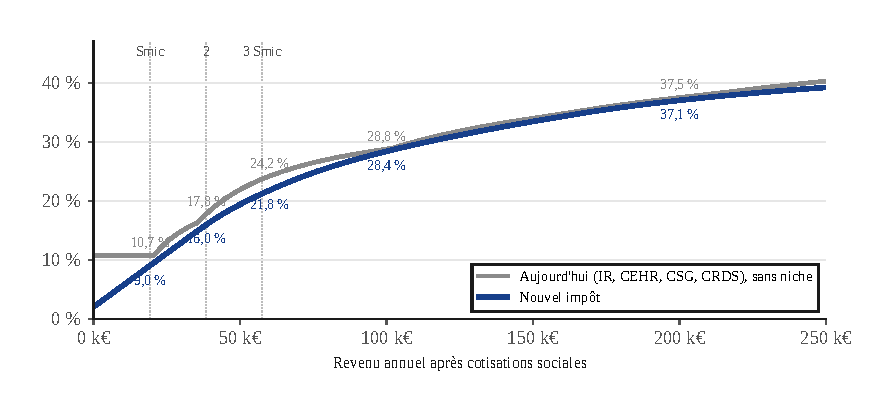
\includegraphics[width=\linewidth]{figures/g1_taux_moyens.pdf}\par
{\raggedright\scriptsize\color{gris}Source : OpenFisca-France 176.1 (droit des revenus 2025) ; calculs des auteurs (note8p/calculs/ircsg4\_*.py).\par Salarié vivant seul, sans enfant, sans niche ni frais réels. Repères : 1 Smic = 19 200 € de revenu après cotisations (21 600 € brut par an, 2025).
\par}\end{minipage}\hfill
\begin{minipage}[t]{0.44\linewidth}\captionsetup{type=table}\caption{Le nouvel impôt : quatre taux, pour chaque adulte,
sur tous ses revenus}\label{tab:bareme}\vspace{4pt}
\small\begin{tabular}{@{}lr@{}}\toprule
Revenu annuel après cotisations & Taux marginal \\ \midrule
jusqu'à 12\,000~€ & 5~\% \\
de 12\,000 à 36\,500~€ & 20~\% \\
de 36\,500 à 120\,000~€ & 28~\% \\
au-delà de 120\,000~€ & 45~\% \\ \midrule
Franchise par enfant & 6\,000~€ \\
Taux maximal aujourd'hui & 52 à 56~\% \\ \bottomrule
\end{tabular}\par\vspace{3pt}
{\raggedright\scriptsize\color{gris}Remplace l'IR, la CSG, la CRDS et la CEHR sur les revenus du travail, les pensions,
le chômage, les bénéfices des indépendants et les revenus fonciers ; les revenus du capital mobilier restent au
prélèvement forfaitaire unique. Seuil de 36\,500~€ calé sur la recette de 2025.\par}
\end{minipage}
\end{figure}

\textbf{La fusion naïve ne suffit pas.} On pourrait se contenter d'ajouter la CSG au barème de l'IR, en relevant tous
ses taux de 4,3 points sur une assiette élargie. On garderait alors les marches de l'IR et un taux maximal proche de
50~\% (figure~\ref{fig:g2}) : une simplification administrative, pas une meilleure fiscalité.

\textbf{Notre proposition : un nouvel impôt, à progressivité modérée.} Chaque adulte paie sur son revenu après
cotisations sociales, quelle qu'en soit l'origine : 5~\% jusqu'à 12\,000~€, 20~\% jusqu'à 36\,500~€, 28~\% jusqu'à
120\,000~€, 45~\% au-delà. Quatre taux, aucune décote, aucun seuil qui fasse basculer tout le revenu : l'impôt et le
revenu disponible sont continus partout. Le taux maximal, CEHR comprise, tombe de 52-56~\% à 45~\% ; un taux de 20~\%
s'applique sans interruption de 0,6 à 1,9 Smic, là où l'empilement actuel culmine. Notre salarié augmenté garde
désormais 80~\% de son augmentation au lieu de 76~\%. Le prix de cette continuité est réel : entre 0,6 et 1,1 Smic, le
taux marginal monte de 10,7 à 20~\%, même si l'impôt total y baisse légèrement. L'épargne retraite reste déductible.
Les autres réductions et crédits d'impôt disparaissent, sauf ceux liés à l'invalidité et à la dépendance ; garder ceux
pour l'emploi à domicile et la garde d'enfants (8,8~Md€) coûterait 0,6 point sur tous les taux.

\graphique{g2_taux_marginaux}{Le taux marginal ne dépasse plus 45~\%, contre 52 à 56~\% aujourd'hui en haut, et
l'escalier de l'impôt sur le revenu disparaît}{fig:g2}

\textbf{Un impôt individuel.} Dans l'imposition commune, le conjoint d'un salarié bien payé est taxé au taux marginal
du couple dès son premier euro. Prenons un couple où l'un gagne 35\,000~€ brut et où l'autre envisage de reprendre un
mi-temps au Smic. Aujourd'hui, l'impôt du foyer augmente de 1\,242~€, soit 11,5~\% de ce second salaire. Avec l'impôt
individuel, de 479~€, soit 4,4~\%. Les études le confirment de longue date : la décision de travailler des seconds
apporteurs de revenu, le plus souvent des femmes, est l'une des plus sensibles à l'impôt. Le revers est clair : un
couple sans enfant à un seul revenu de 80\,000~€ paierait 3\,600~€ de plus. L'individualisation se heurte aussi au
Conseil constitutionnel, qui a censuré en 2012 une contribution individuelle sur les revenus d'activité au nom de
l'égalité entre foyers (décision 2012-662 DC). Nous raisonnons ici sur l'architecture souhaitable. Une étape
intermédiaire existe : un quotient conjugal plafonné à 2\,000~€ d'avantage, qui protège les couples à un revenu mais
taxe le second salaire à 18~\% au lieu de 4~\%. Des règles simples empêchent les transferts artificiels entre conjoints :
salaire du conjoint au prix du marché, revenus des biens communs partagés par moitié.

\textbf{Les enfants comptent.} Un parent qui gagne 50\,000~€ et élève deux enfants n'a pas la même capacité
contributive qu'un célibataire au même revenu. Chaque enfant donne droit à une franchise de 6\,000~€, déduite par le
parent qui a le revenu le plus élevé : c'est le choix qui réduit le plus l'impôt du couple, et il ne touche jamais au
taux du second apporteur, taxé à 5~\% dès son premier euro. Le montant est le même pour chaque enfant. Qu'une
déduction profite davantage à une famille aisée ne nous gêne pas : elle mesure une charge réelle dans un impôt
progressif.

\textbf{Une pension est un revenu comme un autre.} Il n'existe pas de raison générale de taxer moins un revenu parce
qu'il vient d'une caisse de retraite plutôt que d'un employeur. L'abattement de 10~\% (5,3~Md€), les taux réduits de
CSG, l'abattement pour les plus de 65 ans et la demi-part des anciens combattants disparaissent ; les dispositifs liés
à l'invalidité et à la dépendance restent. Les retraités paient 12,9~Md€ de plus, 3,1~\% de leurs pensions, ce qui
finance 11,3~Md€ de baisse pour les actifs. La protection des petites pensions passe par le taux d'entrée de 5~\% et
par le minimum vieillesse, pas par une franchise propre qui recréerait des seuils. L'alignement corrige aussi une
incitation perverse : à 63 ans, une année de travail de plus est aujourd'hui taxée à 29~\% de ce qu'elle rapporte en
plus de la pension ; elle le serait à 19,5~\%.

\graphique{g3_cas_types}{Les familles et les actifs paient moins ; les petites pensions et les familles mono-actives
aisées paient plus}{fig:g3}

\textbf{Regardons maintenant ce que cela change} (figure~\ref{fig:g3}). Un couple de deux actifs avec deux enfants et
60\,000~€ de salaires gagne 1\,100~€ par an ; une famille de quatre enfants vivant d'un salaire de 45\,000~€, 2\,900~€ ;
un parent isolé au Smic avec deux enfants, 1\,700~€. Le cadre supérieur à 120\,000~€ gagne 6\,500~€, et le 1~\% le plus
aisé 2,2~Md€ au total : c'est la conséquence assumée d'un taux maximal de 45~\%. Les perdants sont les retraités
modestes et moyens : +600~€ pour une pension de 12\,000~€, +1\,400~€ à 16\,000~€, alors que les retraités aisés gagnent ;
et, effet de l'individualisation, les familles mono-actives au-delà de 50\,000~€ (+1\,080~€ à 60\,000~€). Pour les
salariés modestes, le gain est faible : 25~€ au Smic, 140~€ à 2\,000~€ net. La réforme améliore leurs incitations plus
que leur revenu.

\textbf{La principale incertitude.} Le gain d'efficacité de la fusion suppose que les salariés réagissent aujourd'hui
à la CSG comme à l'impôt sur le revenu. Le nouvel impôt, publié avec un barème, sera vu en entier ; si la CSG, prélevée
sur la fiche de paie, passe aujourd'hui inaperçue, la fusion rend visible un prélèvement caché. La perte sèche évitée
vaut 3,8~Md€ par an (1,9 à 9,0) si la CSG est perçue comme l'IR, rien si elle ne l'est qu'à moitié, et la réforme
coûte 3,3~Md€ si elle ne l'est pas du tout. Aucune étude ne tranche. Dans le premier cas, environ 300\,000 personnes de
plus voudraient travailler (de 120\,000 à 610\,000), surtout des seconds apporteurs et des temps partiels. La réforme se
défend aussi sans ce gain : un même impôt pour un même revenu, un taux maximal raisonnable, un second salaire moins
taxé, une année de travail en plus mieux récompensée.

\section{Taxer le sol plutôt que les déménagements}

Prenons un couple de trentenaires qui achète son premier appartement à Massy, dans l'Essonne : un trois-pièces de
65~m² au prix médian de la commune, 269\,000~€. Il paie 15\,620~€ de droits de mutation, 5,81~\% du prix, avant les
émoluments du notaire. Primo-accédant, il échappe à la majoration à 5~\% votée par le département jusqu'en 2028 ;
sans cela, il aurait payé 17\,000~€. Nous divisons ces droits par deux : le couple
conserve 7\,810~€ au moment précis où il constitue son apport et s'installe. La contrepartie, nous l'assumons : sa taxe
foncière augmentera d'environ 475~€ par an. L'économie à l'achat vaut seize ans de cette hausse.

Les droits de mutation sont un mauvais impôt pour une raison simple : ils ne frappent que ceux qui bougent. Le couple
qui attend un enfant, la famille qui suit un emploi, le retraité qui voudrait prendre plus petit paient 5,8~\% du prix
à chaque achat ; le propriétaire qui ne bouge pas ne paie rien. Une famille d'Orléans qui accepte un poste en Essonne et
achète une maison de 365\,000~€ à Sainte-Geneviève-des-Bois paie 21\,190~€ de droits : pour les rembourser, il lui faut
une augmentation nette de 294~€ par mois pendant six ans. Les études étrangères montrent que ces droits réduisent la
mobilité résidentielle des propriétaires (Finlande, Royaume-Uni, Pays-Bas) ; aucune étude française ne le mesure, et
aucune ne montre d'effet sur l'emploi. Les effets sur les ventes sont certains à court terme (les ventes ont bondi de
26~\% le mois précédant la hausse de 2014) et disputés à long terme. Quant à la construction, le neuf paie déjà des
droits réduits : la baisse ne la relancera pas mécaniquement.

La taxe foncière, elle, est une bonne assiette mal calculée. Assise sur des valeurs locatives de 1970, elle pèse 0,54~\%
de la valeur d'un logement dans les communes les moins chères et 0,18~\% dans les plus chères (figure~\ref{fig:g4}). Et
elle taxe surtout le bâti, c'est-à-dire ce que le propriétaire a construit, plutôt que le sol, dont la valeur doit tout
à la ville qui l'entoure.

\graphique{g5_achats}{Diviser les droits par deux fait économiser de 5\,000 à 11\,000~€ à l'achat, contre 300 à
650~€ de taxe foncière en plus par an}{fig:g5}

\textbf{Notre proposition : une taxe, une base, deux taux.} Chaque bien reçoit une seule base : la valeur de son
terrain, bâti ou non, plus le quart de la valeur de ses constructions. Le sol est ainsi taxé quatre fois plus que le
bâti. Le contribuable paie le taux voté par sa commune, qui garde sa recette, et un taux national uniforme d'environ
0,20~\% de la valeur du sol. La valeur du sol est fixée par zone à partir des ventes observées, comme dans le
Bade-Wurtemberg, qui taxe depuis 2025 la seule valeur des terrains : surface × valeur de zone, contestable par
expertise au-delà de 30~\% d'écart. Le modèle a été validé par la cour fédérale des finances en mai 2026, mais il a
fallu plus de quatre ans pour évaluer les terrains. Le double taux vient de Pennsylvanie : Pittsburgh l'a pratiqué de
1913 à 2001. Ses effets mesurés sont positifs mais modestes : environ deux à trois points de croissance de plus par
décennie du nombre de logements pour un rapport de quatre entre les taux (Banzhaf et Lavery, 2010).

\deuxgraphiques{g4_taxe_valeur}{Rapportée à la valeur du logement, la taxe foncière pèse trois fois plus dans les communes bon marché}{fig:g4}%
{g6_sol_bati}{Taxer le sol plutôt que le bâti divise par deux l'impôt dû pour avoir construit}{fig:g6}

Pourquoi faisons-nous cela ? Un impôt sur le bâti pénalise celui qui construit ; un impôt sur le sol pénalise celui qui
garde un terrain cher inutilisé (figure~\ref{fig:g6}). Sur un terrain de 200\,000~€, élever un immeuble de 600\,000~€
coûte aujourd'hui 2\,150~€ d'impôt de plus par an ; avec deux taux, 980~€. Laisser le terrain vide coûte 1\,300~€ au
lieu de 720~€.

\textbf{Une hausse nette, assumée.} Nous levons 15~Md€ de taxe foncière nouvelle, quand la baisse des droits en coûte
8,1. L'excédent, environ 5,5~Md€ par an, finance la baisse de l'impôt sur les sociétés. Les impôts périodiques sur
l'immobilier passeraient de 1,9 à 2,4~\% du PIB, entre la moyenne de l'OCDE et le Royaume-Uni. La hausse moyenne est de
300~€ par logement et par an (237~€ pour la moitié des logements), plus forte là où le sol est cher : +850~€ pour
l'appartement parisien médian. La hausse de la taxe se reporte dans les prix : les propriétaires actuels perdent à
l'annonce environ 3,6~\% de la valeur de leur logement (322~Md€ au total). Faut-il les compenser ? Non. Une partie de la
valeur d'un terrain n'est que la capitalisation d'une rente foncière peu taxée ; la compenser reviendrait à annuler la
réforme. L'acheteur suivant, lui, paie moins cher et ne perd rien. Une perte de patrimoine n'est pas une difficulté de
trésorerie : un retraité modeste dans une maison qui a pris de la valeur peut ne pas pouvoir payer 500~€ de plus. Il
pourra reporter la hausse, avec intérêt, jusqu'à la vente ou à la succession. Ce prêt est compté : 0,2 à 0,6~Md€ par an.

\textbf{Pas de baisse à crédit.} L'ancienne version de cette réforme baissait les droits tout de suite et montait la
taxe ensuite ; c'était la principale source de dette de transition. Désormais, les deux avancent ensemble : la part
nationale de la taxe monte par tiers en 2029, 2030 et 2031, et les droits baissent le 1\textsuperscript{er} janvier des
mêmes années, de 5,81 à 4,84, 3,87 puis 2,90~\%. Une clause suspend chaque baisse tant que la taxe correspondante n'est
pas en recouvrement. Des acheteurs attendront un palier, mais un palier ne fait gagner qu'un point de droits : le
décalage reste de quelques semaines. À terme, si les recettes et le marché le permettent, la suppression complète des
droits pourra être envisagée.

\section{Favoriser les entreprises qui investissent et grandissent}

Prenons une PME industrielle qui achète une machine de 500\,000~€ en juillet. Amortie sur sept ans, elle ne peut en
déduire que 35\,714~€ la première année. Avec notre réforme, elle déduit tout de suite la moitié du prix, puis amortit
l'autre moitié normalement : 267\,857~€ la première année. Elle garde 58\,000~€ de trésorerie de plus, qu'elle rendra
les années suivantes. L'avantage réel, actualisé, est de 9\,500~€. C'est beaucoup plus qu'une baisse du taux : pour une
machine qui rapporte juste ce qu'elle coûte, deux points de taux en moins ne valent que 1\,700~€.

Pourquoi ? Une baisse du taux allège l'impôt sur tous les bénéfices, y compris ceux des investissements déjà faits et
des rentes. La déduction immédiate ne profite qu'à l'investissement nouveau. Les évaluations les plus solides vont dans
ce sens. Aux États-Unis, la déduction anticipée de 30 à 50~\% a accru l'investissement des entreprises concernées de
10 à 17~\%, deux fois plus chez les petites (Zwick et Mahon, 2017). Au Royaume-Uni, des amortissements de première année
plus généreux ont relevé le taux d'investissement des entreprises moyennes d'environ 11~\% (Maffini, Xing et Devereux,
2019). Le bilan de la réforme américaine de 2017 conclut que la déduction immédiate a livré la moitié de
l'accumulation de capital de la baisse du taux pour un tiers de son coût (Chodorow-Reich, Zidar et Zwick, 2024).

\textbf{Notre combinaison.} \emph{D'abord, la fin du taux réduit.} Les sociétés de moins de 10~M€ de chiffre d'affaires
paient 15~\% sur leurs 42\,500 premiers euros de bénéfice : un avantage de 4\,250~€ au plus, qui va à toute petite
société, qu'elle investisse ou non, holdings patrimoniales comprises. La petite taille est un mauvais indicateur des
difficultés de financement, et cet avantage n'est pas un obstacle macroéconomique : sa suppression se défend par la
neutralité et rapporte 2,7~Md€. \emph{Ensuite, la déduction immédiate de 50~\% des équipements neufs}, introduite à
25~\% en 2028. \emph{Enfin, la baisse du taux normal} à 24~\% en 2030, 23~\% en 2033 et 22,5~\% en 2035, au rythme des
recettes. Le taux facial des grands groupes passerait de 25,8 à environ 23,2~\%, sous la moyenne de l'OCDE (24,2~\%) :
c'est ce taux, plus que l'amortissement, qui compte pour l'implantation des entreprises et des bénéfices.

\graphique{g7_tmei}{Notre combinaison divise par deux l'impôt sur l'investissement marginal, pour un coût permanent
proche de celui de la seule baisse du taux}{fig:g7}

Combien cela coûte-t-il ? Il faut distinguer deux choses. La déduction avance l'impôt sans l'effacer : son coût est
élevé les premières années (jusqu'à 6,7~Md€), puis tombe à 0,7~Md€ par an, une fois que les machines achetées après la
réforme n'ont plus que la moitié de leur prix à amortir. Les « 5~Md€ » de la variante étudiée naguère étaient une dette
de transition, pas un coût annuel. La déduction intégrale aurait coûté 14,8~Md€ la première année, pour un effet par
euro identique : on pourrait aller plus loin, mais est-ce la meilleure utilisation de nos ressources fiscales tant que
le budget ne le permet pas ? Au total, le capital productif augmenterait d'environ 11~Md€ (5,6 à 18,7) et le PIB
potentiel d'environ 0,06~\% à long terme (0,03 à 0,10) : un gain réel mais modeste, qu'il ne faut pas survendre.

Il y a des perdants. Une petite société de services qui investit peu perd le taux réduit sans profiter de la
déduction : à 60\,000~€ de bénéfice, elle paiera 2\,750~€ de plus par an au taux de 22,5~\% ; elle perd tant que son
bénéfice est inférieur à 170\,000~€. Et la déduction favorise les activités qui achètent des équipements ; les services
investissent surtout en logiciels, déjà amortis en deux ou trois ans, et en bâtiments, que seule la baisse du taux
aide. D'où la combinaison. Enfin, nous ne créons pas de biais nouveau en faveur de la dette : l'avantage de l'emprunt
sur les fonds propres recule un peu, et une machine financée pour un tiers par emprunt reste taxée à peu près à zéro,
contre un taux négatif de 13~\% avec la déduction intégrale.

\textbf{Pour aller plus loin.} La déduction intégrale, la neutralité entre dette et fonds propres (sur le modèle de
l'abattement belge ou italien), un meilleur traitement des pertes sont des orientations souhaitables à terme. Elles
coûtent cher pour des effets moins établis ; nous ne les retenons pas aujourd'hui.

\section{Une fiscalité du capital plus neutre et plus stable}

Nous ne touchons pas au prélèvement forfaitaire unique de 31,4~\%. Le baisser coûterait 0,4 à 0,7~Md€ par point, et
la baisse de 2018 a surtout accru les dividendes versés, sans effet mesurable sur l'investissement ni sur les salaires
(France Stratégie, 2023). Nous préférons concentrer nos ressources sur des mesures mieux documentées, et offrir aux
épargnants ce qui leur a le plus manqué : la stabilité.

Nous corrigeons en revanche une anomalie. Prenons un entrepreneur qui a constitué une société pour 100\,000~€ ; ses
titres valent aujourd'hui un million. S'il vend, il paie 282\,600~€ sur sa plus-value, puis son enfant paie des droits
de succession sur le reste : 410\,800~€ au total. S'il garde ses titres jusqu'à sa mort, l'enfant paie 213\,000~€ de
droits sur le million, puis revend sans impôt, car la plus-value est effacée. Garder jusqu'au décès fait économiser
200\,000~€ : l'impôt incite à ne pas vendre aux âges élevés, et ceux qui le peuvent transmettent plutôt que de céder.

Notre règle : l'héritier ou le donataire reprend le prix d'acquisition d'origine. Rien n'est dû au décès ni à la
donation ; la plus-value accumulée est imposée quand il vend, et jamais s'il ne vend pas. Pour éviter une double
imposition, les droits de succession payés sur la plus-value latente s'ajoutent au prix repris, comme aux États-Unis
pour les donations. Dans notre exemple, l'héritier qui revend paie au total 435\,000~€, à peu près ce qu'aurait payé son
parent en vendant (figure~\ref{fig:g9}). C'est une hausse effective de l'impôt de certains patrimoines, que nous
assumons ; elle est forte pour les entreprises transmises sous pacte Dutreil, dont la charge passe de 3 à 30~\% si
l'héritier revend, sans rien changer à la transmission elle-même.

\graphique{g9_exemple_pv}{Transmettre efface aujourd'hui la moitié de l'impôt ; avec la réforme, l'héritier paie à peu
près ce qu'aurait payé le parent en vendant}{fig:g9}

Trois précautions. La règle s'applique dès son annonce, sinon chaque année d'attente laisse passer une vague de
donations anticipées. Elle vaut pour les plus-values déjà accumulées : le fait générateur reste la vente future,
mais le risque constitutionnel devra être expertisé, et une date de référence à l'annonce en est la solution de repli.
Elle ne supprime pas tout verrouillage : l'héritier, comme tout détenteur, hésitera à vendre une plus-value ; mais la
prime à garder jusqu'à la mort disparaît. Les recettes, enfin, arrivent lentement, quand les héritiers vendent : 0,9~Md€
en 2028, 2,1 en 2030, 3,7 en 2040 au centre, de 1 à près de 10~Md€ selon les hypothèses. Nous ne les dépensons pas
avant de les avoir constatées. À plus long terme, l'indexation des plus-values sur l'inflation et le rapprochement des
régimes de placement seraient souhaitables ; ils ne sont ni simples ni gratuits.

\section{Une réforme financée, au service de la croissance}

\graphique{g8_bouclage}{Les pensions financent la baisse de l'impôt des actifs ; le sol finance la baisse des droits et
celle de l'impôt sur les sociétés}{fig:g8}

\textbf{D'où vient l'argent, où va-t-il ?} (figure~\ref{fig:g8}). Le nouvel impôt sur le revenu est à recette
constante : l'alignement des pensions (+12,9~Md€) finance la baisse pour les actifs. La nouvelle taxe foncière
(15~Md€) finance la division par deux des droits de mutation (8,1~Md€), le report de paiement et la déductibilité de la
taxe, puis, avec la fin du taux réduit (2,7~Md€), la déduction immédiate et la baisse du taux normal de l'IS. Les
recettes de la fin de l'effacement des plus-values restent en réserve tant qu'elles ne sont pas constatées ; si elles
atteignent le niveau central, elles permettront de descendre vers 21,5~\% d'IS au milieu des années 2030. Au total, l'impôt sur
le revenu baisse pour les actifs et monte pour les retraités ; l'impôt sur le sol monte, celui sur les transactions
baisse ; l'impôt sur les sociétés baisse de 5,4~Md€ par an, dont une partie est reprise aux mêmes entreprises par la
taxe sur leurs terrains.

\textbf{Sans un euro de dette.} Chaque mesure n'entre en vigueur qu'avec sa recette. Le nouvel impôt monte en charge
sur quatre ans, des deux côtés à la fois ; les droits baissent au rythme de la taxe foncière ; la déduction immédiate
attend 2028 et le taux de l'IS ne baisse que lorsque les recettes foncières sont là ; la même clause de suspension
que pour les droits s'applique aux mesures d'IS si la taxe foncière prend du retard. Le solde de l'ensemble reste
compris entre $-0,2$ et $+1,1$~Md€ chaque année de 2027 à 2040, sans compter les plus-values (tableau~\ref{tab:traj}).
Deux évolutions déjà inscrites dans le droit sont distinctes de nos réformes et ne les financent pas : la fin de la
contribution exceptionnelle sur les bénéfices des grandes entreprises (7~Md€ par an de recette en moins, à assumer ou
à compenser) et l'extinction de la CRDS fin 2033, qui permettra de baisser tous les taux du nouvel impôt d'environ
0,5 point.

\begin{table}[!htbp]\centering\small\setlength{\tabcolsep}{3.2pt}
\caption{Aucune année de déficit : solde des quatre réformes (Md€ de 2027, + = recette en plus)}\label{tab:traj}
\begin{tabular}{@{}lrrrrrrrrr@{}}
\toprule
 & 2027 & 2028 & 2029 & 2030 & 2031 & 2032 & 2033 & 2035 & 2040 \\
\midrule
Foncier net (taxe − droits − report) & 0,0 & $-$0,5 & 2,1 & 3,8 & 5,8 & 5,2 & 5,2 & 5,3 & 5,5 \\
Fin du taux réduit d'IS & 0,0 & 1,3 & 2,7 & 2,7 & 2,7 & 2,7 & 2,7 & 2,7 & 2,7 \\
Déduction immédiate & 0,0 & 0,0 & $-$3,7 & $-$6,6 & $-$5,1 & $-$3,9 & $-$3,0 & $-$1,3 & $-$0,7 \\
Baisse du taux normal & 0,0 & 0,0 & 0,0 & 0,0 & $-$2,8 & $-$2,8 & $-$4,3 & $-$5,9 & $-$7,4 \\
Taux normal de l'IS (exercice précédent) & 25 & 25 & 25 & 25 & 24 & 24 & 23,5 & 23 & 22,5 \\
\textbf{Solde} & \textbf{0,0} & \textbf{0,8} & \textbf{1,0} & $\mathbf{-0,1}$ & \textbf{0,6} & \textbf{1,1} &
\textbf{0,6} & \textbf{0,7} & \textbf{0,0} \\
\emph{Réserve : fin de l'effacement, si constatée} & 0,0 & 0,9 & 1,9 & 2,1 & 2,3 & 2,5 & 2,6 & 3,0 & 3,7 \\
\bottomrule
\end{tabular}
\par\vspace{2pt}{\raggedright\scriptsize\color{gris}Source : calculs des auteurs (note8p/calculs/bouclage.py). Années
d'encaissement ; l'IS d'un exercice est encaissé l'année suivante. Le nouvel impôt sur le revenu, à recette constante,
pèse $-0,05$~Md€ par an. Détail et sensibilités dans l'annexe technique.\par}
\end{table}

\textbf{Ce que nous pouvons raisonnablement chiffrer.} Nous ne donnons pas de chiffre global de croissance : les
études ne le permettent pas. Pour l'investissement, le calcul est assez solide pour parler de PIB : environ 0,06~\% à
long terme. Pour le travail, environ 300\,000 personnes de plus voudraient travailler et la perte sèche évitée vaut
3,8~Md€ par an, à condition que la CSG soit aujourd'hui perçue comme un impôt ; sinon, ce gain disparaît. Pour
l'immobilier, la perte sèche évitée vaut 2,5~Md€ par an si les ventes réagissent durablement aux droits, 0,8~Md€ sinon.
La perte sèche mesure l'activité que l'impôt fait renoncer à entreprendre, pas un supplément de PIB (annexe technique).

Notre conviction tient en quelques phrases. Travailler davantage doit rapporter davantage. Les charges de famille
doivent être reconnues. Une pension ne doit pas être mieux traitée qu'un salaire. Il faut moins taxer les
déménagements et les constructions, davantage la rente foncière. Il faut favoriser les entreprises qui investissent et
grandissent plutôt que celles qui restent petites. Et tout cela peut se faire sans augmenter les prélèvements ni la
dette. Il ne s'agit pas de construire la fiscalité mathématiquement parfaite, mais une fiscalité française
sensiblement plus favorable à la prospérité.

\end{document}
